\clearpage
\section{BB84 with Discrete Variables}

\begin{tcolorbox}	
\begin{tabular}{p{2.75cm} p{0.2cm} p{10.5cm}} 	
\textbf{Students Name}  &:& Mariana Ramos and Kevin Filipe\\
\textbf{Starting Date} &:& November 7, 2017\\
\textbf{Goal}          &:& BB84 implementation with discrete variables.
\end{tabular}
\end{tcolorbox}

BB84 is a key distribution protocol which involves three parties, Alice, Bob and Eve. Alice and Bob exchange information between each other by using a quantum channel and a classical channel. The main goal is continuously build keys only known by Alice and Bob, and guarantee that eavesdropper, Eve, does not gain any information about the keys.


\subsection{Protocol Analysis}
\begin{tcolorbox}	
	\begin{tabular}{p{2.75cm} p{0.2cm} p{10.5cm}} 	
		\textbf{Students Name}  &:& Kevin Filipe (7/11/2017 - 10/11/2017)\\
		\textbf{Goal}          &:& BB84 - Protocol Description
	\end{tabular}
\end{tcolorbox}

BB84 protocol was created by Charles Bennett and Gilles Brassard in 1984 \cite{BB84}. It involves two parties, Alice and Bob, sharing keys through a quantum channel in which could be accessed by a eavesdropper, Eve. A basic model is depicted in figure \ref{fig:qkd model}.

\begin{figure}[H]
	\centering
	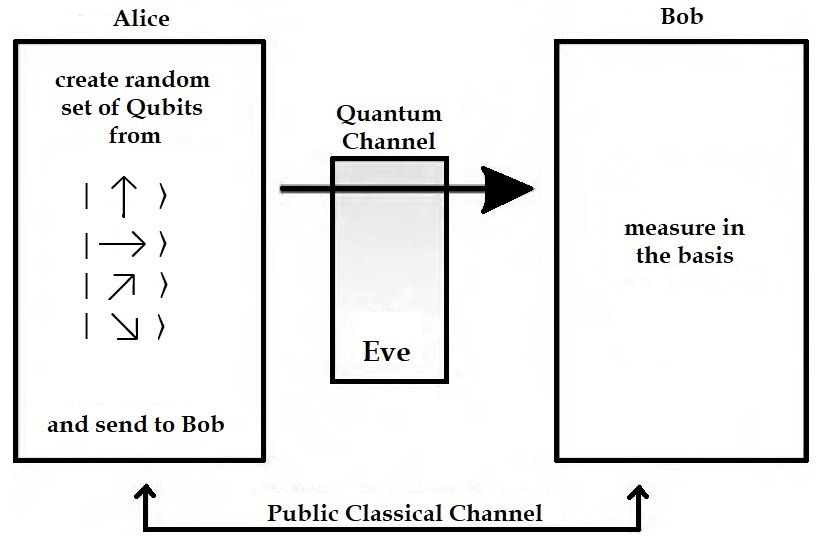
\includegraphics[width=0.8\textwidth,height=7cm]{./sdf/bb84_with_discrete_variables/figures/QKD_Model.png}
	\caption{Basic QKD Model. Alice and Bob are connected by 2 communication channels, a public quantum channel and a authenticated classical channel, with an eavesdropper, Eve (figure adapted from \cite{iqo}).}\label{fig:qkd model}
\end{figure}

We are going to analyse the BB84 protocol with bit encoding into photon state polarization. Two non-orthogonal basis are used to encode the information, the rectilinear and diagonal basis, + and x respectively. The following table shows this bit encoding.
\begin{table}[H]
	\centering
	\begin{tabular}{c|c|c}
		 Bit &  \textit{Rectilinear Basis,+} & \textit{Diagonal Basis,$\times$}\\ \hline
		0 &  0$º$ & -45$º$ \\
		1 & 90$º$ & 45$º$\\
	\end{tabular}
\end{table}

The protocol requires the following parameter and it is implemented with the following steps:

\begin{table}[hbt]
	\centering
	\caption{Initial Parameters.}
	\label{tb:param}
	\begin{tabular}{|c|c|}
		\hline
		\textbf{Parameter}  & \textbf{Description} 	   \\ \hline
			$M \times N$    & Scrambling Matrix M by N \\ \hline
			k				& Number of revealed bits for BER calculation \\ \hline
			$\alpha$        & Confidence level 	       \\ \hline
			    A    & B                \\ \hline
	\end{tabular}
\end{table}

\begin{enumerate}
	\item Alice generates two random bit strings. The random string , $R_{A1}$, corresponds to the data to be encoded into photon state polarization. $R_{A2}$ is a random string in which 0 and 1 corresponds to the rectilinear, +, and diagonal, $\times$, respectively.
	
	$$ R_{A1} = \{0,1,1,0,1,0,0,1,1,0,1,1,1,0,0,1,0,0,0,1\}$$
	\begin{eqnarray}
		R_{A2} &=& \{0,0,1,0,1,1,1,0,1,1,1,0,1,0,0,0,1,0,1,0\} \nonumber \\
		&=& \{+,+,\times,+,\times, \times, \times, +,\times, \times, \times,+,\times,+,+,+,\times,+,\times,+\}\nonumber
	\end{eqnarray}
	
	\item Alice transmits a train of photons, $S_{AB}$, obtained by encoding the bits, $R_{A1}$ with the respective photon polarization state $R_{A2}$.
	
	$$S_{AB} = \{\to, \uparrow, \searrow, \to, \searrow, \nearrow, \nearrow, \uparrow, \searrow, \nearrow, \searrow, \uparrow, \searrow, \to, \to, \uparrow, \nearrow, \to, \nearrow, \uparrow\}.$$
	
	\item Bob generates a random string, $R_{B}$, to receive the photon trains with the correspondent basis.
	\begin{eqnarray}
		R_{B} &=& \{0,1,1,1,0,1,0,0,1,1,0,0,1,1,0,0,1,1,0,0\} \nonumber\\
		&=&\{+,\times,\times,\times,+,\times,+,+,\times,\times,+,+,\times,\times,+,+,\times,\times,+,+\} \nonumber
	\end{eqnarray}
	
	\item Bob performs the incoming photon states measurement, $M_{B}$, with its generated random basis, $R_{B}$. If the two photon detectors don't click, means the bit was lost during transference due to attenuation. If both photon detectors click, a false positive was detected. In the measurements, $M_{B}$, the no-click in both detectors is represented by a -1 and the false positives to -2. The measurements done in rectilinear or diagonal basis are represented by 0 or 1, respectively. This is represented \ref{fig:bb84 detector}
	
	$$M_{B} = \{0,1,1,1,-1,1,0,0,-2,1,0,0,-2,1,0,0,1,-1,0,0\}$$	

	\begin{figure}[H]
		\centering
		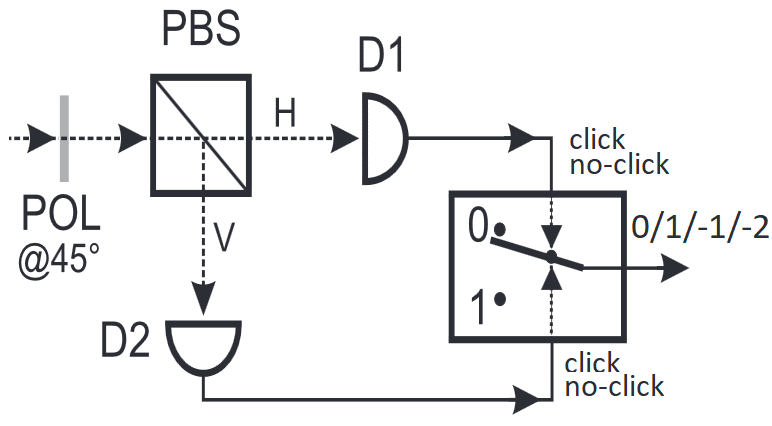
\includegraphics[width=0.8\textwidth,height=7cm]{./sdf/bb84_with_discrete_variables/figures/detector.png}
		\caption{Photon Detection block with false-positives, -2, and attenuation, -1, detection depending on D1 and D2 output.\label{fig:bb84 detector}}
	\end{figure}
	
	\item After the measurement, Bob sends to Alice, using the classical channel, the used basis values, $R_{B}$ with the attenuation, -1, and false positives,-2.
	\item Alice performs a modified negated XOR, generating a sequence that detects when the same basis she used $B_{AB}$.
	
	\begin{table}[H]
		\centering
		\begin{tabular}{c|c c c c c c c c c c c c c c c c c c c c}
			$R_{A2}$ & 0 & 0 & 1 & 0 &  1 & 1 & 1 & 0 &  1 & 1 & 1 & 0 &  1 & 0 & 0 & 0 & 1 &  0 & 1 & 0 \\
			$R_{B}$  & 0 & 1 & 1 & 1 & -1 & 1 & 0 & 0 & -2 & 1 & 0 & 0 & -2 & 1 & 0 & 0 & 1 & -1 & 0 & 0 \\ \hline
			$B_{AB}$ & 1 & 0 & 1 & 0 &  0 & 1 & 0 & 1 &  0 & 1 & 0 & 1 &  0 & 0 & 1 & 1 & 1 &  0 & 0 & 1 \\
		\end{tabular}
	\end{table}

	\item Alice sends the $B_{AB}$ sequence to Bob, in which he can correlate with, $M_{B}$, and deduce the key $K_{AB}$.
	
			$$ K_{AB} = \{0,1,0,1,0,1,0,1,0,1\}.$$
	
	\item Alice then by having knowledge of $R_{A2}$ and $B_{AB}$ performs a scrambling algorithm over the deduced key. It is generated a matrix $M \times N$, according to the input parameter. Assuming a scrambling matrix of 3x4, \ref{tb:scram}. And being the scramble key represented as $KS_{AB}$
	
	\begin{table}[hbt]
		\centering
		\caption{Scrambling matrix}
		\label{tb:scram}
		\begin{tabular}{|c|c|c|c|c|}
			\hline
				0 & 1 & 0 & 1 \\ \hline
			    0 & 1 & 0 & 1 \\ \hline
				0 & 1 & - & - \\ \hline
		\end{tabular}
	\end{table}

	$$KS_{B} = \{0,0,0,1,1,1,0,0,1,1\}$$	
	
	\item Bob uses the same algorithm as Alice and scrambles his key.
	
	\item Bob then reveals a fixed number of his key to Alice. This number is also an input parameter value, k. With this the Quantum Bit Error Rate (QBER).
		
\end{enumerate}

	To determine the QBER, it is necessary to know the confidence interval parameter, $\alpha$ and the QBER limit, in which states the maximum allowed QBER by the user.
	Then to verify if the channel is reliable or not, the flowchart presented in figure \ref{fig:flowQber}.
	
	\begin{enumerate}
		\item Bob will reveals k bits sequence from the scrambled key, $SK_{AB}$ to Alice.
		\item Alice then returns to Bob the estimated QBER value, mQBER, with a confidence interval, [qLB, qUB] using the using the equations in the Bit Error Rate section, but applied to this protocol
		\item To check if the channel is compromised or not it is necessary to check if the QBER limit is higher than the QBER upper bound. If QBER limit is between the QBER lower and upper bound it is necessary to reveal more k bits from the key. Otherwise the channel is compromised and the key determination process needs to restart.
	\end{enumerate}
	
	
\begin{figure}[H]
	\centering
	\includegraphics[width=1\textwidth,height=7cm]{./sdf/bb84_with_discrete_variables/figures/qberEstimation.png}
	\caption{Flowchart to determine if the channel is reliable or not.}\label{fig:flowQber}
\end{figure}



\newpage

\subsection{Simulation Analysis}

\begin{tcolorbox}	
\begin{tabular}{p{2.75cm} p{0.2cm} p{10.5cm}} 	
\textbf{Students Name}  &:& Mariana Ramos (7/11/2017 - 12/1/2018) \\
\textbf{Goal}          &:& Perform a simulation of BB84 communication protocol.
\end{tabular}
\end{tcolorbox}

In this sub section the simulation setup implementation will be described in order to implement the BB84 protocol. In figure \ref{toplevelsimulation} a top level diagram is presented. Then it will be presented the block diagram of the transmitter block (Alice) in figure \ref{alicesimulation}, the receiver block (Bob) in figure \ref{bobsimulation} and finally the eavesdropper block (Eve) in figure \ref{evesimulation}.

\begin{figure}[H]
	\centering
	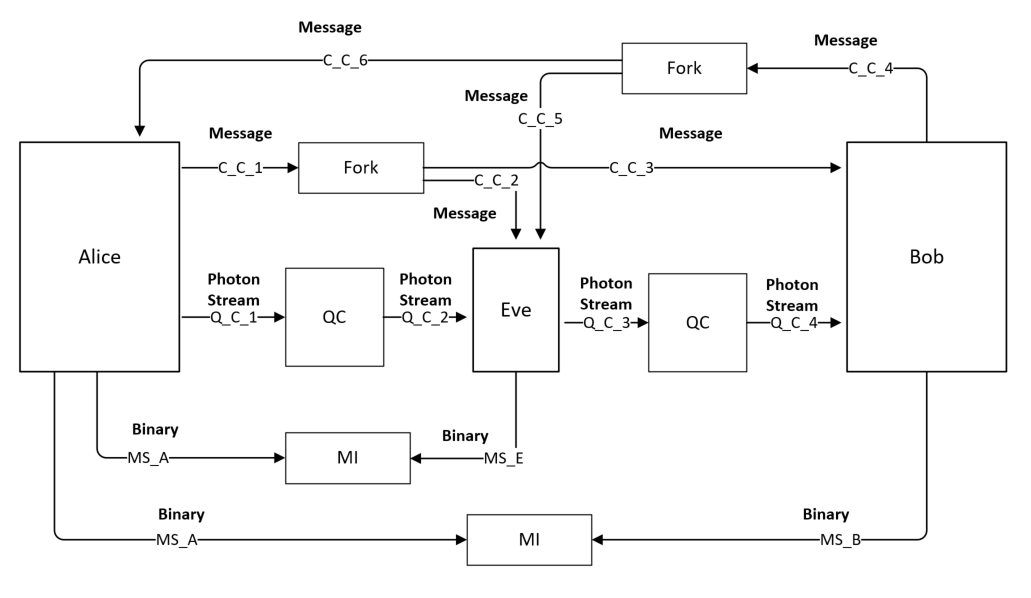
\includegraphics[width=1.0\textwidth, height=9cm]{./sdf/bb84_with_discrete_variables/figures/toplevel_simulation.png}
	\caption{Simulation diagram at a top level}\label{toplevelsimulation}
\end{figure}

Figure \ref{toplevelsimulation} presents the top level diagram of our simulation. The setup contains three parties, Alice, Eve and Bob where the communication between them is done throughout two authenticated classical channels and one public quantum channel. In the middle of the classical channel there is a Fork's diagram which has one input and two outputs. In the case of the classical channel \textbf{C\_C\_4} which has the information sent by Bob, the fork's block enables Alice and Eve access it. In the quantum communication, the information sent by Alice can be intercepted by Eve and changed by her, or can follow directly to Bob as we can see later in figure \ref{evesimulation}. Furthermore, for mutual information calculation there must be two blocks \textbf{MI}, one to calculate the mutual information between Alice and Eve, and other to calculate the mutual information between Alice and Bob.

\begin{figure}[h]
    \centering
        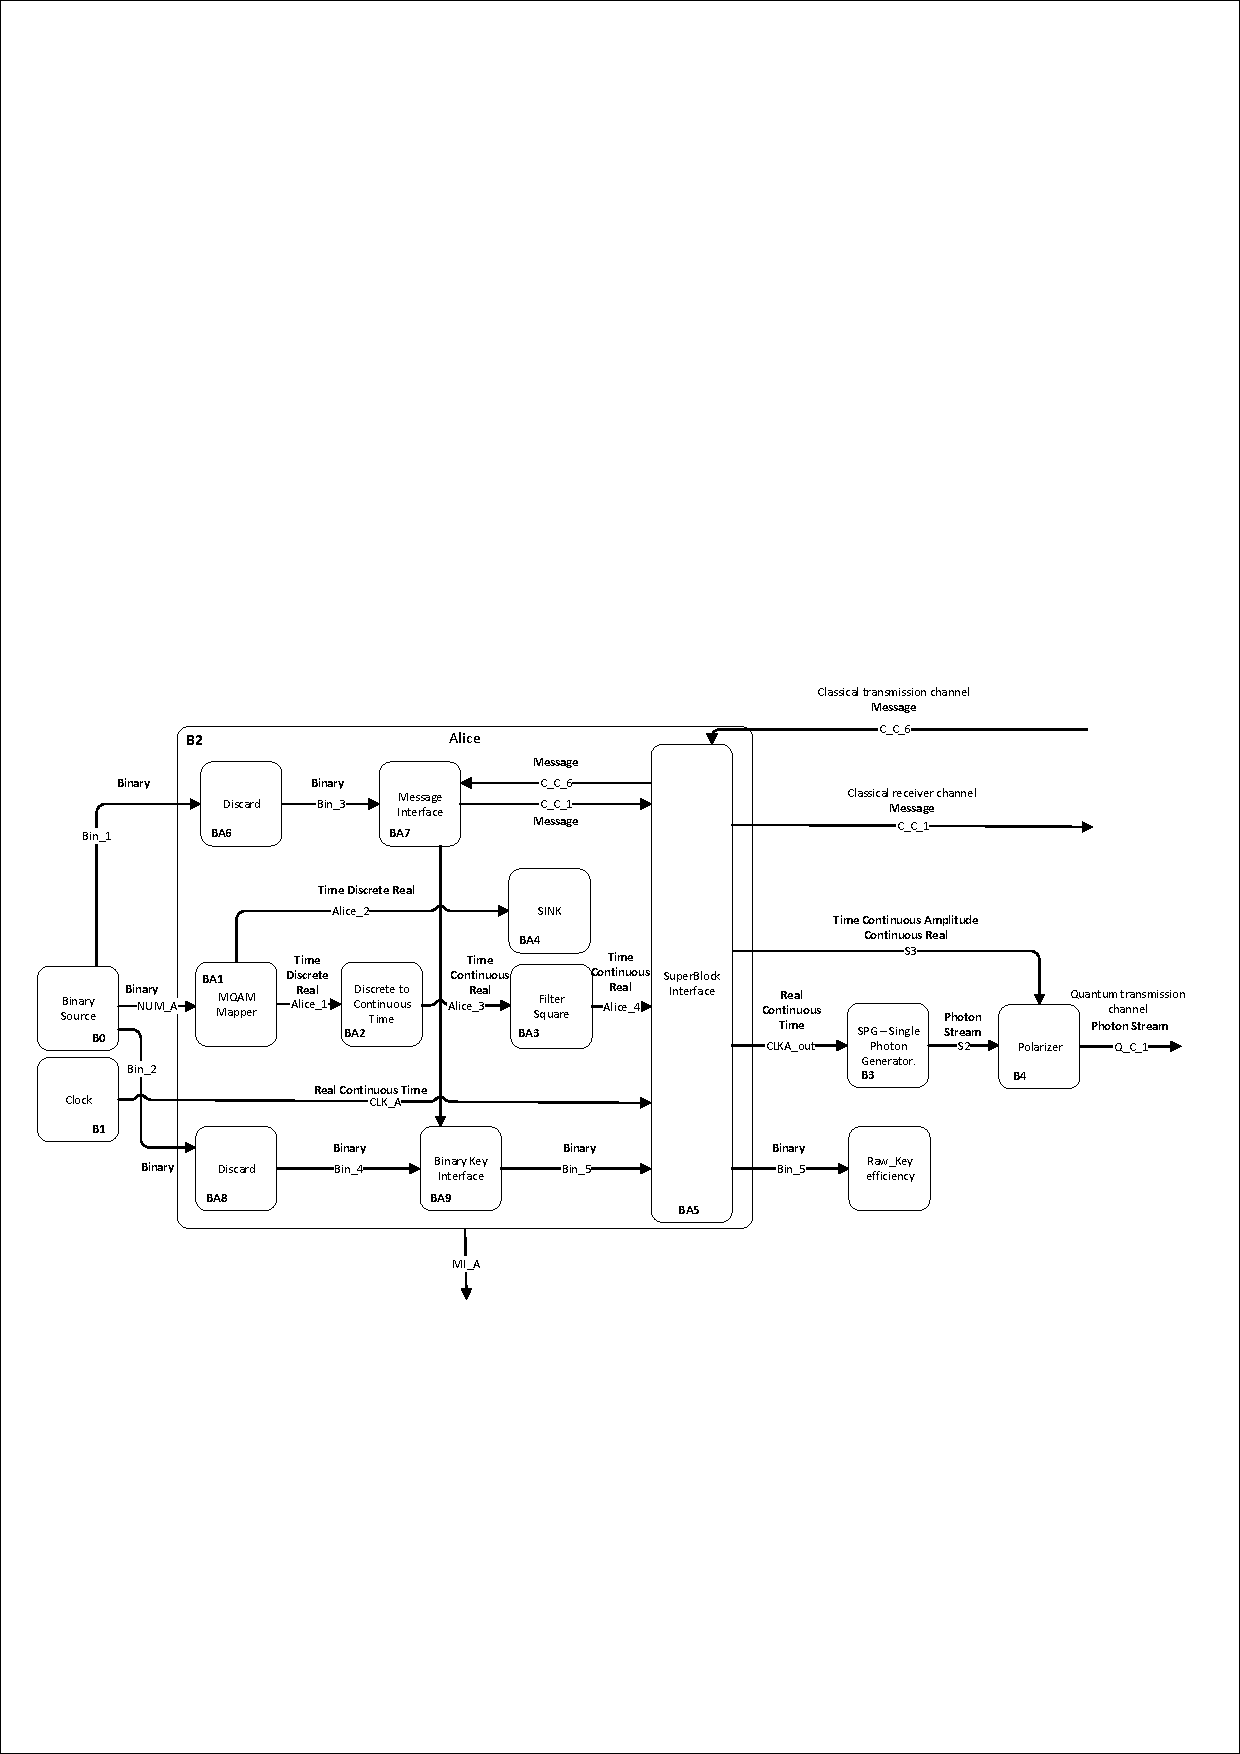
\includegraphics[clip, trim=0.5cm 6cm 0.5cm 10cm, width=1.00\textwidth]{./sdf/bb84_with_discrete_variables/figures_raw/Simulation_Alice_bb84.pdf}
    \caption{Simulation diagram at Alice's side}\label{alicesimulation}
\end{figure}


\begin{figure}[h]
    \centering
        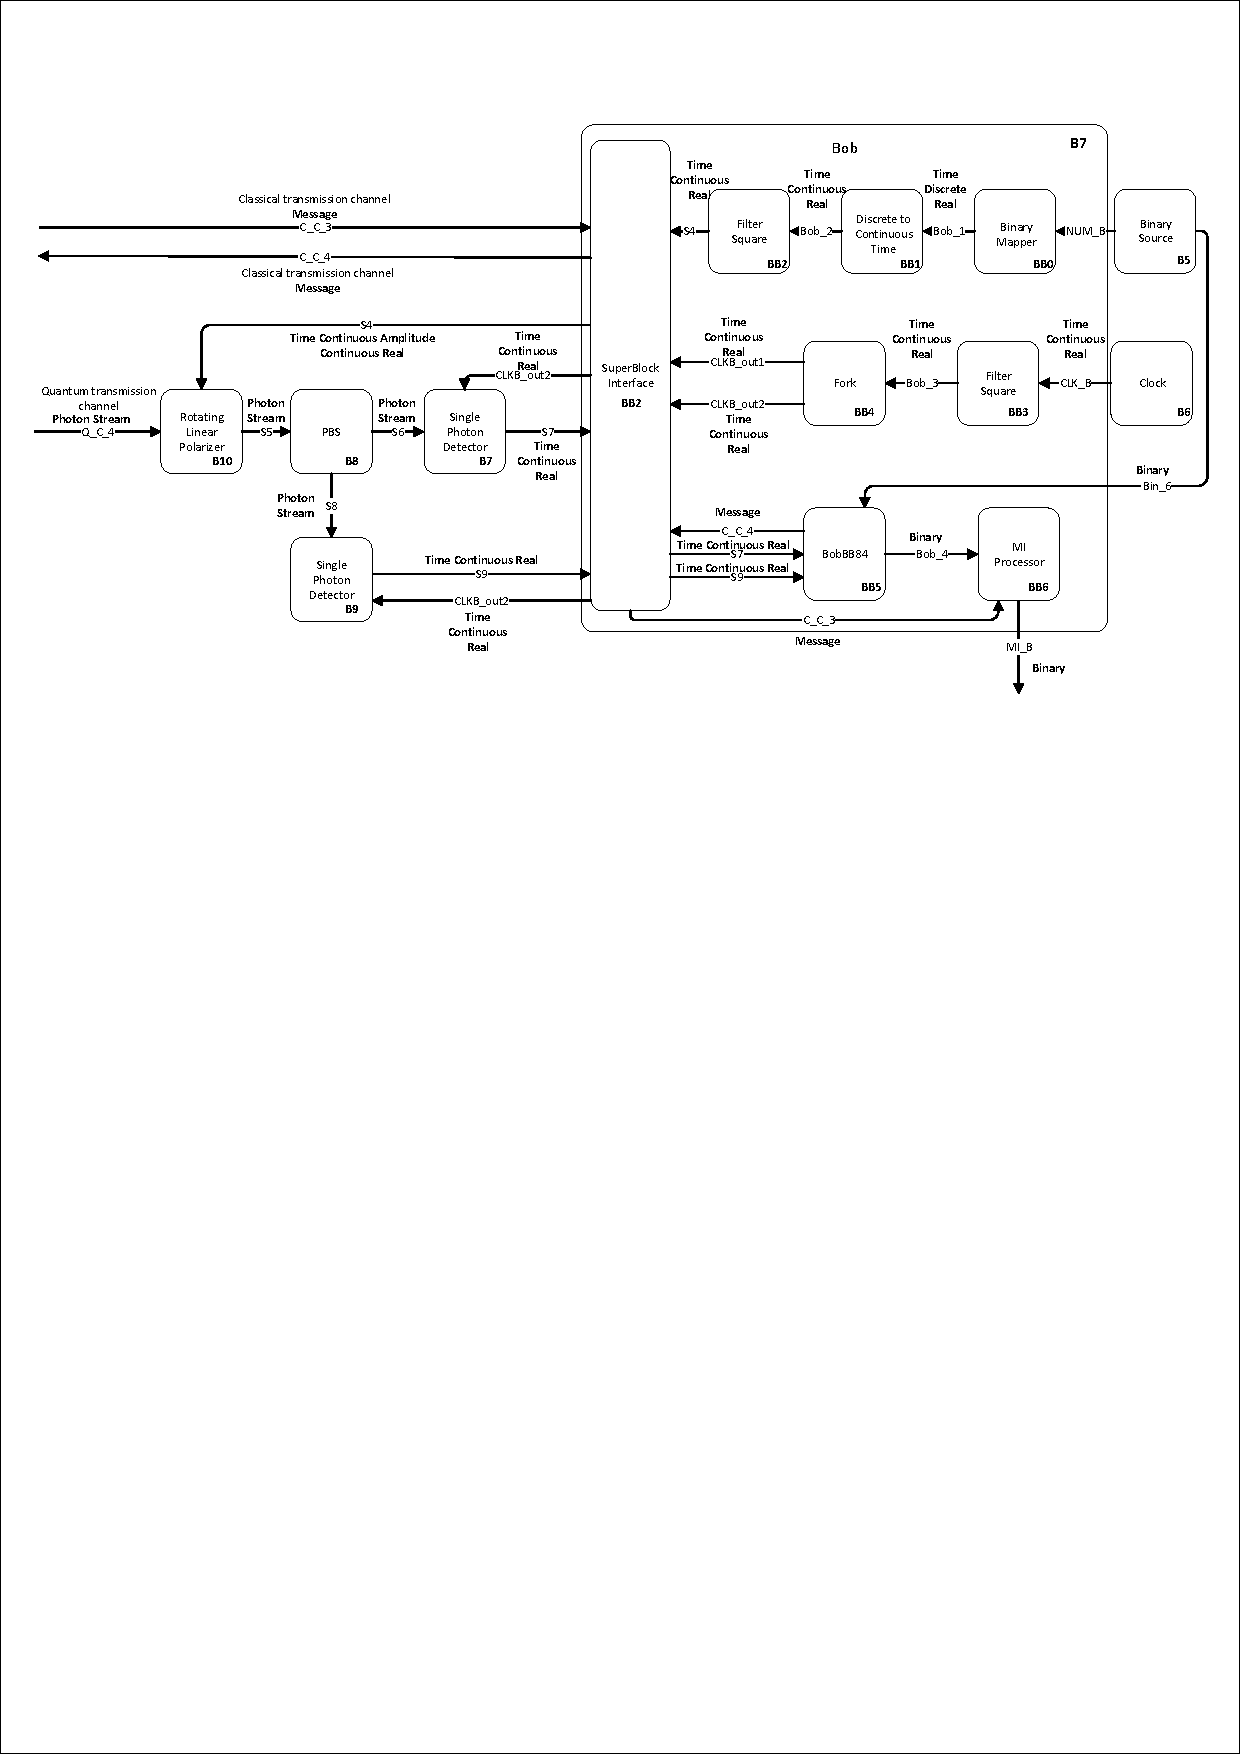
\includegraphics[clip, trim=0.5cm 16cm 0.5cm 2cm, width=1.00\textwidth]{./sdf/bb84_with_discrete_variables/figures_raw/Simulation_Bob_bb84.pdf}
    \caption{Simulation diagram at Bob's side}\label{bobsimulation}
\end{figure}

    In figure \ref{alicesimulation} one can observe a block diagram of the simulation at Alice's side. As it is shown in the figure, Alice must have one block for random number generation which is responsible for basis generation to polarize the photons, and for key random generation in order to have a random state to encode each photon. Furthermore, she has a Processor block for all logical operations: array analysis, random number generation requests, and others. This block also receives the information from Bob after it has passed through a fork's block. In addition, it is responsible for set the initial length $l$ of the first array of photons which will send to Bob. This block also must be responsible for send classical information to Bob. Finally, Processor block will also send a real continuous time signal to single photon generator, in order to generate photons according to this signal, and finally this block also sends to the polarizer a real discrete signal in order to inform the polarizer which basis it should use. Therefore, she has two more blocks for quantum tasks: the single photon generator and the polarizer block which is responsible to encode the photons generated from the previous block and send them throughout a quantum channel from Alice to Bob.

    Finally, Alice's processor has an output to Mutual Information top level block, $Ms_{A}$.

    In figure \ref{alicesimulation} one can observe a block diagram of the transmitter. As it is shown in the figure, the transmitter must have one block for random number generation (binary source) which is responsible for basis generation to polarize the photons, and for key random generation in order to have a random state to encode each photon. This block has three outputs which will be inputs for the super block Alice. Furthermore, Alice block is responsible for all logical operations: random single photons state values generation, receive and send messages to the receiver Bob by using the classical channels, binary output for mutual information calculations. Each block of the super block is described in Library chapter. Finally, Alice block will also send a real continuous time signal to single photon generator (clock sets the rate oh photons generation), in order to generate photons polarized in the horizontal axis by default. Therefore, the transmitter has one more block, the polarizer block, which is responsible to encode the photons generated from the previous block and send them throughout a quantum channel from Alice to Bob.

     In figure \ref{bobsimulation} one can see a block diagram of the simulation for receiver (Bob). The receiver has one block for Random Number Generation which is responsible for randomly generate basis values which Bob will use to measure the photons sent by Alice throughout the quantum channel. Like transmitter, the receiver has the Bob block responsible for receive and send messages through the classical channel, receive single photons values detection from the single photon detectors, provides a clock signal to the detectors and send binary values for mutual information calculation. Furthermore, the receiver has two blocks for single photon detection (one for horizontal detection and other for vertical detection) which receives from Bob block a real continuous time signal which will set the detection window for the detector and outputs for Bob block the result value for detection. In addition, there is a polarizer which receives from Bob block a time continuous real signal which provides information about the rotation angle. If the basis chosen by Bob is the diagonal basis he sends $45º$, otherwise sends "0º". The polarization beam splitter divides the input photon stream in horizontal component and vertical component.




\begin{figure}[h]
	\centering
	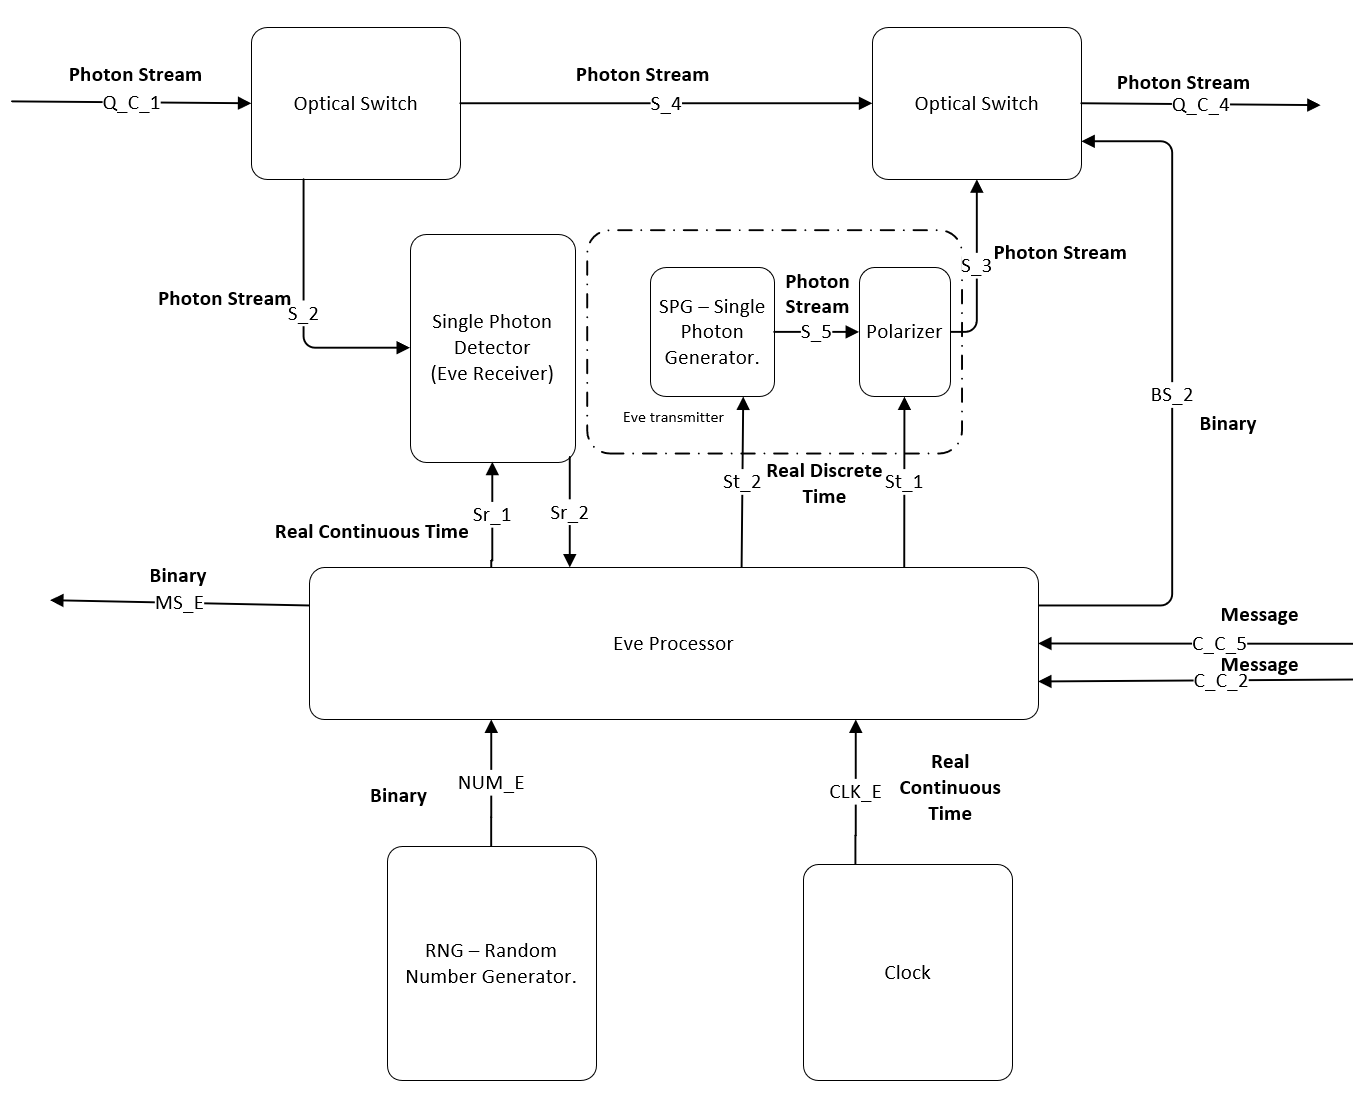
\includegraphics[width=1.1\textwidth, height=14cm]{./sdf/bb84_with_discrete_variables/figures/eve_simulation.png}
	\caption{Simulation diagram at Eve's side}\label{evesimulation}
\end{figure}

Figure \ref{evesimulation} presents the Eve's side diagram. Eve's processor has two receiver classical signals, one from Alice (\textbf{C\_C\_2}) and other from Bob (\textbf{C\_C\_5}). About quantum channel, Eve received a quantum message from Alice through the channel \textbf{Q\_C\_1} and depends on her decision the photon can follows directly to Bob or the photon's state can be changed by her. In this case, the photon is received by a block similar to Bob's diagram \ref{bobsimulation} and this block sends a message to Eve's processor in order to reveal the measurement result. After that, Eve's processor sends a message to Alice's diagram similar to figure \ref{alicesimulation} and this block is responsible for encode the photon in a new state. Now, the changed photon is sent to Bob.

In addition, Eve's diagram has one more output $Ms_{E}$ which is a message sent to the mutual information block as an input parameter.

\begin{table}[H]
\centering
\caption{System Signals}
\label{tb:signals}
\begin{tabular}{|c|c|c|}
\hline
\textbf{Signal name}                        & \textbf{Signal type}                      \\ \hline
NUM\_A, NUM\_B, Bin\_1, Bin\_2, Bin\_6      &  Binary                                   \\ \hline
MI\_A, MI\_B                                &  Binary                                   \\ \hline
CLK\_A, CLK\_B                              &  TimeContinuousAmplitudeContinuous        \\ \hline
CLK\_A\_out, CLKB\_out1, CLKB\_out2         &  TimeContinuousAmplitudeContinuous        \\ \hline
S2, S5, S6, S8                              &  PhotonStreamXY                           \\ \hline
S3, S7, S9                                  &  TimeContinuousAmplitudeDiscreteReal      \\ \hline
S4                                          &  TimeContinuousAmplitudeContinuousReal      \\ \hline
C\_C\_1, C\_C\_3                            &  Messages                                 \\ \hline
C\_C\_6, C\_C\_4                            &  Messages                                 \\ \hline
Q\_C\_1, Q\_C\_4                            &  PhotonStreamXY                           \\ \hline

\end{tabular}
\end{table}

Table \ref{tb:signals} presents the system signals as well as them type.

\begin{table}[H]
\centering
\caption{System Input Parameters}
\label{tb:inputparameters}
\begin{tabular}{|c|c|c|}
\hline
\textbf{Parameter}                      & \textbf{Default Value}                                & \textbf{Description} \\ \hline
RateOfPhotons                           & 1K                                                    &                 \\ \hline
vector<t\_iqValues> iqAmplitudeValues   & \{-45.0,0.0\},\{0.0,0.0\},\{45.0,0.0\},\{90.0,0.0\}   &                 \\ \hline

\end{tabular}
\end{table}

\begin{table}[H]
\centering
\caption{Header Files}
\label{tb:signals}
\begin{tabular}{|c|c|c|}
\hline
\textbf{File name}                              & \textbf{Description} & \textbf{Status} \\ \hline
netxpto.h                                       &                      &    \checkmark   \\ \hline
alice\_qkd.h                                    &                      &  Working on     \\ \hline
binary\_source.h                                &                      &    \checkmark   \\ \hline
bob\_qkd.h                                      &                      &   Working on    \\ \hline
clock\_20171219.h                               &                      &    \checkmark   \\ \hline
discrete\_to\_continuous\_time.h                &                      &    \checkmark   \\ \hline
eve\_qkd.h                                      &                      &   Missing       \\ \hline
m\_qam\_mapper.h                                &                      &    \checkmark   \\ \hline
optical\_switch.h                               &                      &   Missing       \\ \hline
polarization\_beam\_splitter\_20180109.h        &                      &  Working on     \\ \hline
polarizer.h                                     &                      &    \checkmark   \\ \hline
pulse\_shaper.h                                 &                      &     \checkmark  \\ \hline
single\_photon\_detector.h                      &                      &    \checkmark   \\ \hline
single\_photon\_source\_20171218.h              &                      &    \checkmark   \\ \hline
sink.h                                          &                      &    \checkmark   \\ \hline
super\_block\_interface.h                       &                      &    \checkmark   \\ \hline
message\_processor\_alice.h                     &                      &    Working on   \\ \hline
demux\_1\_2.h                                   &                      &    \checkmark   \\ \hline
scrambling.h                                    &                      &    Missing      \\ \hline
binary\_mapper.h                                &                      &    \checkmark   \\ \hline
bobBB84.h                                       &                      &    Missing      \\ \hline
message\_processor\_bob.h                       &                      &    Missing      \\ \hline
\end{tabular}
\end{table}

\begin{table}[H]
\centering
\caption{Source Files}
\label{tb:signals}
\begin{tabular}{|c|c|c|}
\hline
\textbf{File name}                                  & \textbf{Description} & \textbf{Status} \\ \hline
netxpto.cpp                                         &                      &    \checkmark   \\ \hline
bb84\_with\_discrete\_variables.cpp                 &                      &  Working on     \\ \hline
alice\_qkd.cpp                                      &                      &  Working on     \\ \hline
binary\_source.cpp                                  &                      &    \checkmark   \\ \hline
bob\_qkd.cpp                                        &                      &   Missing       \\ \hline
clock\_20171219.cpp                                 &                      &    \checkmark   \\ \hline
discrete\_to\_continuous\_time.cpp                  &                      &    \checkmark   \\ \hline
eve\_qkd.cpp                                        &                      &   Missing       \\ \hline
m\_qam\_mapper.cpp                                  &                      &    \checkmark   \\ \hline
optical\_switch.cpp                                 &                      &   Missing       \\ \hline
polarization\_beam\_splitter\_20180109.cpp          &                      &  Working on     \\ \hline
polarizer.cpp                                       &                      &  Working on     \\ \hline
pulse\_shaper.cpp                                   &                      &     \checkmark  \\ \hline
rotator\_linear\_polarizer.cpp                      &                      &  Working on     \\ \hline
single\_photon\_detector.cpp                        &                      &   Missing       \\ \hline
single\_photon\_source\_20171218.cpp                &                      &    \checkmark   \\ \hline
sink.cpp                                            &                      &    \checkmark   \\ \hline
super\_block\_interface.cpp                         &                      &    \checkmark   \\ \hline
message\_processor\_alice.cpp                       &                      &    Working on   \\ \hline
demux\_1\_2.cpp                                     &                      &    \checkmark   \\ \hline
scrambling.cpp                                      &                      &    Missing      \\ \hline
binary\_mapper.cpp                                  &                      &    \checkmark   \\ \hline
bobBB84.cpp                                         &                      &    Missing      \\ \hline
message\_processor\_bob.cpp                         &                      &    Missing      \\ \hline
\end{tabular}
\end{table}

\subsection{Open Issues}

There still are some open issues in simulation code.

One of them was detected in block \textbf{single\_photon\_source\_20171218.cpp}. This block should assume each sample with 4 real values, since it writes two complex values each time the block runs, i.e each \textit{bufferput()} should write an array of two complex values in outputSignal, outputSignals[0]->bufferPut(valueXY), where \textit{t\_complex\_xy valueXY = \{valueX, valueY\}} and \textit{t\_complex valueX = (realValue\_1,realValue\_2)}. This way, independently of the number of samples these four values should always be written. However, if we chose a number of samples which is not divisible by 4, the four numbers are not written in the last "sample" and the array data for X's values and Y's values have different sizes which is wrong. For example, if we chose 10 samples to acquire, the last values correspond to X's values instead of Y's values and the first array data is longer than the other.

\begin{thebibliography}{2}
	\bibitem{BB84}
	Bennett, C. H. and Brassard,
	G. Quantum Cryptography: Public key distribution and coin tossing.
	International Conference on Computers, Systems and Signal Processing, Bangalore, India, 10-12 December 1984, pp. 175-179.
	
	\bibitem{SURV}
	Mart Haitjema, A Survey of the Prominent Quantum Key Distribution Protocols
	
	\bibitem{iqo}
	Christopher Gerry, Peter Knight, "Introductory Quantum Optics" Cambridge University Press, 2005
	
	\bibitem{SPREADING}
	Varadarajan, S., Ngo, H. Q., \& Srivastava, J. (n.d.). An Adaptive , Perception-Driven Error Spreading Scheme in Continuous Media Streaming.
	
\end{thebibliography}
\cleardoublepage
